% PLANTILLA APA7
% Creado por: Isaac Palma Medina
% Última actualización: 25/07/2021
% @COPYLEFT

% Fuentes consultadas (todos los derechos reservados):  
% Normas APA. (2019). Guía Normas APA. https://normas-apa.org/wp-content/uploads/Guia-Normas-APA-7ma-edicion.pdf
% Tecnológico de Costa Rica [Richmond]. (2020, 16 abril). LaTeX desde cero con Overleaf (1 de 3) [Vídeo]. YouTube. https://www.youtube.com/watch?v=kM1KvHVuaTY Weiss, D. (2021). 
% Formatting documents in APA style (7th Edition) with the apa7 LATEX class. https://ctan.math.washington.edu/tex-archive/macros/latex/contrib/apa7/apa7.pdf @COPYLEFT

%+-+-+-+-++-+-+-+-+-+-+-+-+-++-+-+-+-+-+-+-+-+-+-+-+-+-+-+-+-+-++-+-+-+-+-+-+-+-+-+

% Preámbulo
\documentclass[stu, 12pt, letterpaper, donotrepeattitle, floatsintext, natbib, helv]{apa7}
\usepackage[utf8]{inputenc}
\usepackage{comment}
\usepackage{marvosym}
\usepackage{graphicx}
\usepackage{float}
\usepackage[normalem]{ulem}
\usepackage[spanish]{babel} 
\usepackage{gensymb}
%\usepackage{titling}
\let\apasubparagraph\subparagraph
\let\subparagraph\paragraph
\usepackage[compact]{titlesec}
\let\subparagraph\apasubparagraph
\usepackage{hyperref}
\selectlanguage{spanish}
\useunder{\uline}{\ul}{}
\newcommand{\myparagraph}[1]{\paragraph{#1}\mbox{}\\}
\graphicspath{{./images/}}
\titleformat{\section}{\normalfont\large\bfseries}{\thetitle. \quad }{0pt}{}[{ \titlerule[0.8pt]}]
\titleformat{\subsection}{\normalfont\bfseries}{}{}{}[]

% Portada

\begin{document}
\begin{titlepage}
    \centering
    \vfill
    \LARGE Laboratorio \#9\\
    \vskip2cm
    \large Diego Quirós Artiñano \\
    Universidad Nacional de Costa Rica \\
    EIF-202: Soporte Técnico \\ 
    Carolina Gómez Fernández \\
    07 de junio, 2022 \\
    \vfill
    
\includegraphics[width = 0.4\textwidth]{../../../UNAImage/UNA.png} \\
    \vfill
    \vfill
    % (autores separados, consultar al docente)
    % Manera oficial de colocar los autores:
    %\author{Autor(a) I, Autor(a) II, Autor(a) III, Autor(a) X}
\end{titlepage}

% Índices
\pagenumbering{roman}
    % Contenido
\addto\captionsspanish{
    \renewcommand*\contentsname{\largeÍndice}
}
\tableofcontents
\setcounter{tocdepth}{2}
\newpage
    % Figuras
\renewcommand{\listfigurename}{\largeÍndice de fíguras}
\listoffigures
\newpage
%     % Tablas
% \renewcommand{\listtablename}{\largeÍndice de tablas}
% \listoftables
% \newpage

% Cuerpo
\pagenumbering{arabic}

%------------------------------------------------------------------------------------
\section*{Introducción}
\phantomsection
\addcontentsline{toc}{section}{Introducción}
En este laboratorio se va a hacer el procedimiento de instalar un sistema operativo de Linux desde cero, para esto se va a usar Virtual box para hacerlo dentro de una máquina virtual.

%------------------------------------------------------------------------------------
\section*{Instalación de la máquina virtual}
\phantomsection
\addcontentsline{toc}{section}{Instalación de la máuina virtual}
Después de descargar e instalar virtual box estos son los pasos a seguir para una nueva máquina virtual

\begin{enumerate}
    \item Seleccione el botón de nuevo.
    \begin{figure} [H]
        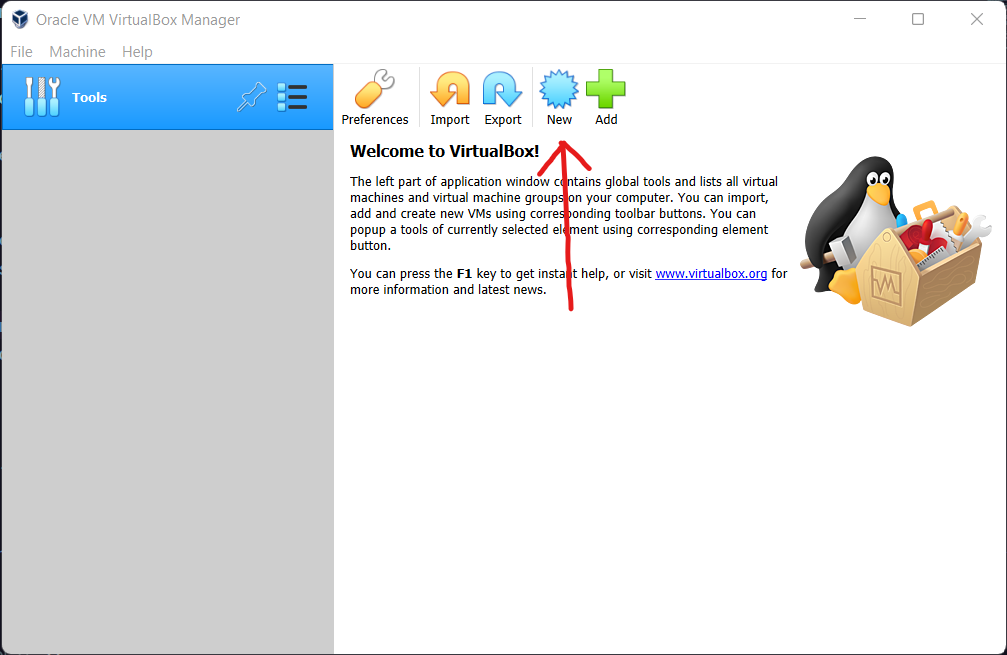
\includegraphics[width = 1\textwidth]{New.png}
        \caption{Creando una nueva máquina virtual}
        \label{fig:New}
    \end{figure}
    \item Seleccione cuanto RAM en MB está dispuesto a permitirle a la máquina virtual utilizar, yo prefiero dejarle como 4GB de RAM.
    \begin{figure} [H]
        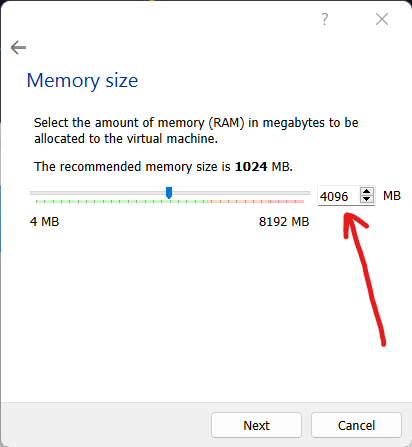
\includegraphics[width = 1\textwidth]{RAMSelection.png}
        \caption{Seleccionando RAM}
        \label{fig:RAM}
    \end{figure}
    \item Seleccionando la versión y el tipo de sistema operativo que quiere usar con la máquina virtual. Personalmente estoy usando Kali Linux que es una distribución basada en Ubuntu y mi computadora soporte sistema operativos de 64-bit entonces eso fue lo que seleccioné.
    \begin{figure} [H]
        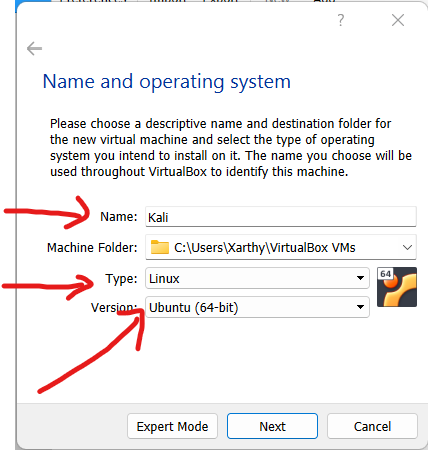
\includegraphics[width = 1\textwidth]{Version.png}
        \caption{Seleccionando Version}
        \label{fig:Version}
    \end{figure}
    \item Creando un disco duro virtual para la máquina virtual. A mi me gusta además alocarlo dinámicamente para que si no lo estoy usando que no se gaste del disco duro de la computadora. Además considero que los 8GB que recomienda son suficientes.
    \begin{figure} [H]
        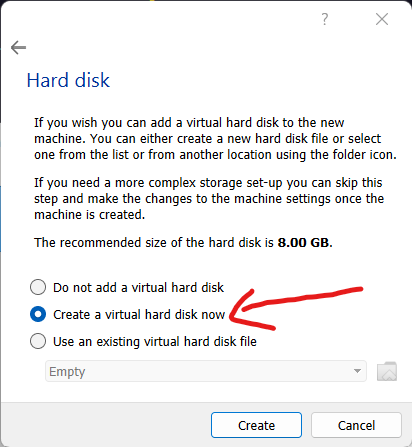
\includegraphics[width = 1\textwidth]{VirtualHardDiskCreation1.png}
        \caption{Alocando espacio para disco duro virtual (1)}
        \label{fig:VHDD1}
    \end{figure}
    \begin{figure}[H]
        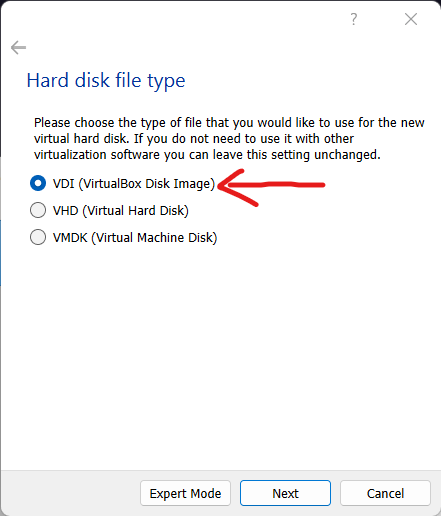
\includegraphics[width = 1\textwidth]{VirtualHardDiskCreation2.png} \\
        \caption{Alocando espacio para disco duro virtual (2)}
        \label{fig:VHDD2}
    \end{figure}
    \begin{figure}[H]
        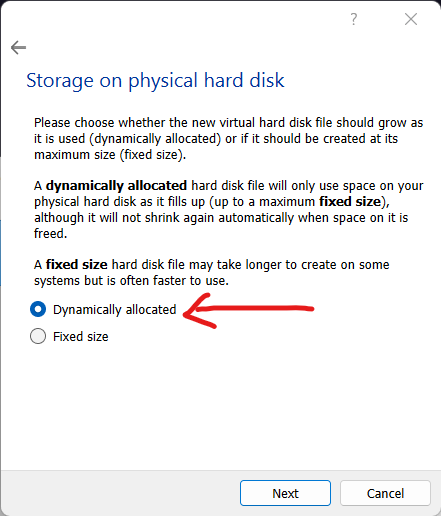
\includegraphics[width = 1\textwidth]{VirtualHardDiskCreation3.png} \\
        \caption{Alocando espacio para disco duro virtual (3)}
        \label{fig:VHDD3}
    \end{figure}
    \begin{figure}[H]
        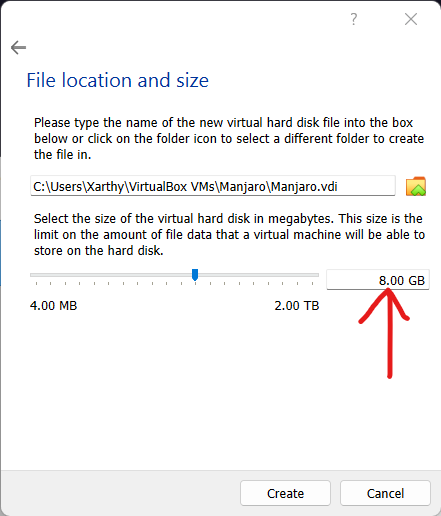
\includegraphics[width = 1\textwidth]{VirtualHardDiskCreation4.png} \\
        \caption{Alocando espacio para disco duro virtual (4)}
        \label{fig:VHDD4}
    \end{figure}
\end{enumerate}

%------------------------------------------------------------------------------------
\section*{Instalación del sistema operativo}
\phantomsection
\addcontentsline{toc}{section}{Instalación del sistema operativo}
Después de la instalación de la máquina virtual se puede instalar el sistema operativo de su preferencia.
\begin{enumerate}
    \item Se selecciona el botón de start.
    \begin{figure} [H]
        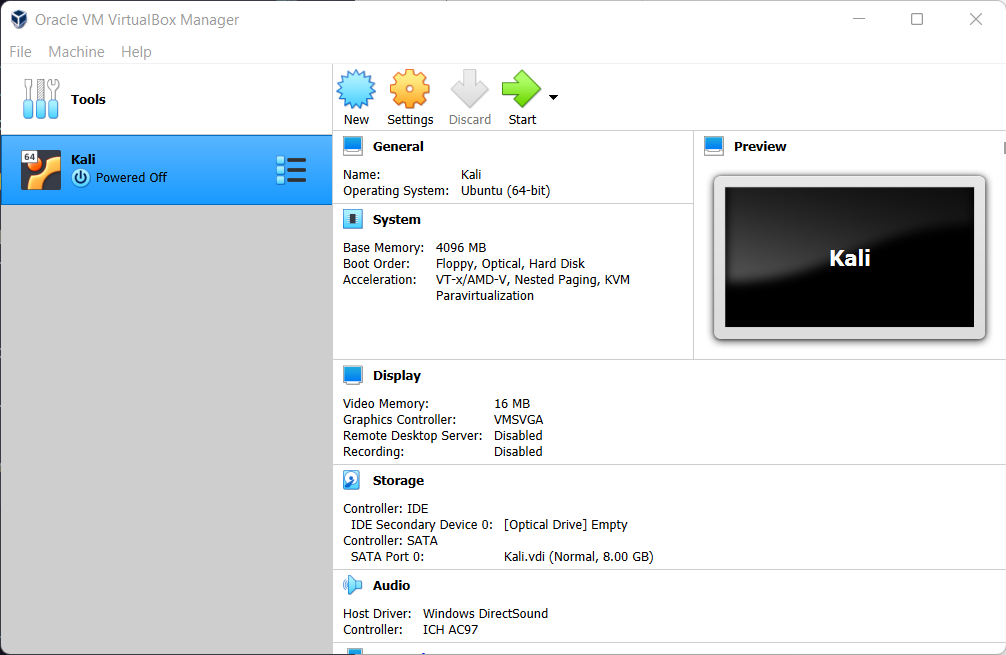
\includegraphics[width = 1\textwidth]{Start.png}
        \caption{Se corre la máquina virtual}
        \label{fig:Start}
    \end{figure}
    \item Se tiene que seleccionar el .iso que quiere utilizar (seleccionar el sistema operativo).
    \begin{figure} [H]
        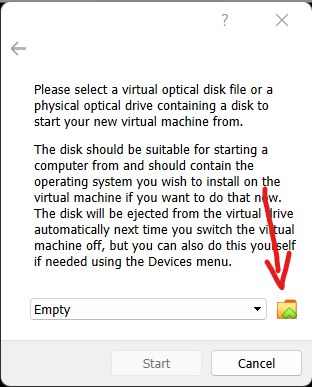
\includegraphics[width = 1\textwidth]{SelectingISO1.png}
        \caption{Seleccionando sistema operativo (1)}
        \label{fig:Select1}
    \end{figure}
    \begin{figure} [H]
        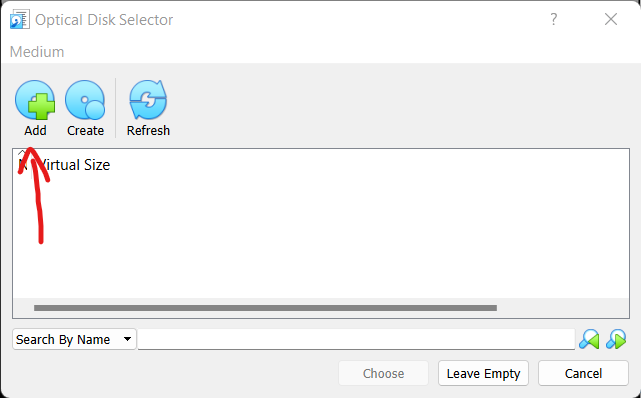
\includegraphics[width = 1\textwidth]{SelectingISO2.png}
        \caption{Seleccionando sistema operativo (2)}
        \label{fig:Select2}
    \end{figure}
    \begin{figure} [H]
        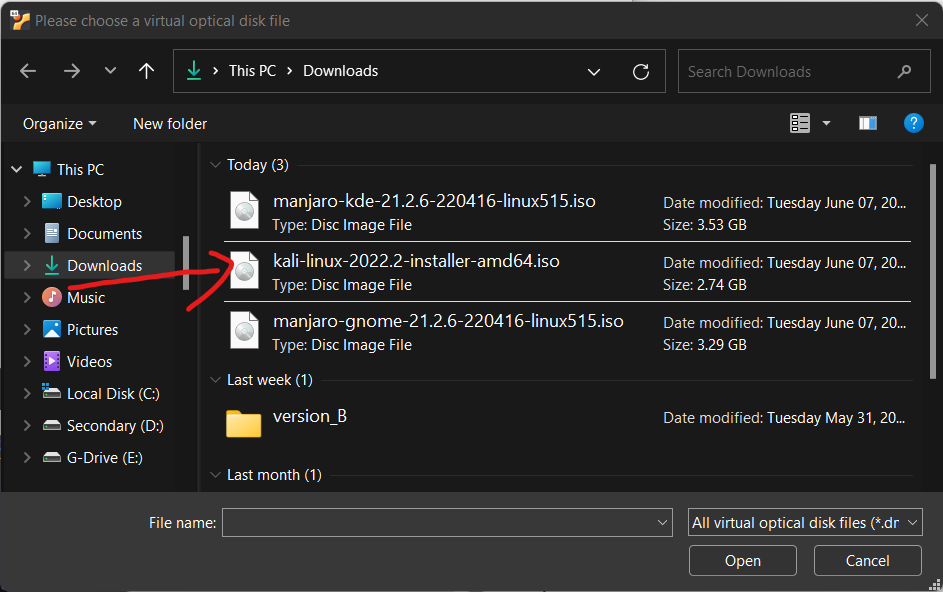
\includegraphics[width = 1\textwidth]{SelectingISO3.png}
        \caption{Seleccionando sistema operativo (3)}
        \label{fig:Select3}
    \end{figure}
    \begin{figure} [H]
        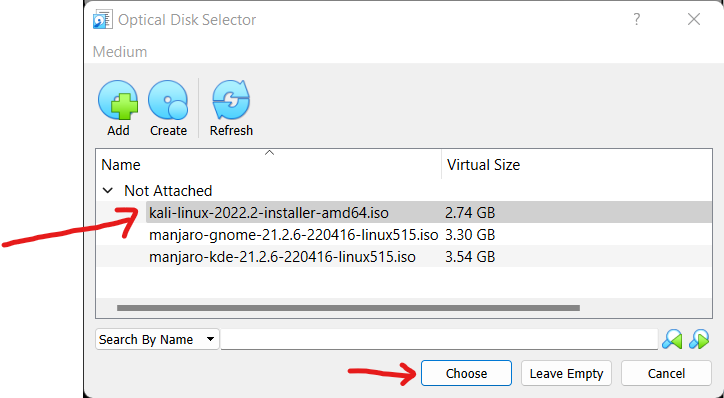
\includegraphics[width = 1\textwidth]{SelectingISO4.png}
        \caption{Seleccionando sistema operativo (4)}
        \label{fig:Select4}
    \end{figure}
    \begin{figure} [H]
        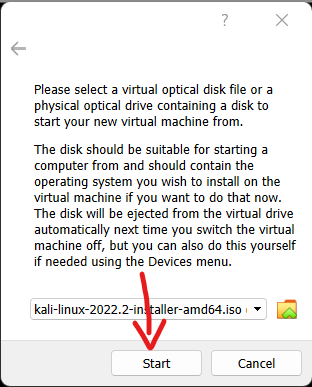
\includegraphics[width = 1\textwidth]{SelectingISO5.png}
        \caption{Seleccionando sistema operativo (5)}
        \label{fig:Select5}
    \end{figure}
    \item Se selecciona como quiere instalar el sistema operativo.
    \begin{figure} [H]
        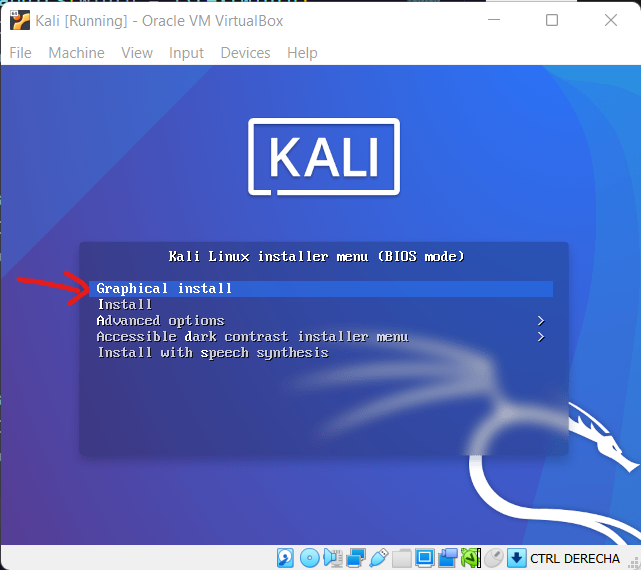
\includegraphics[width = 1\textwidth]{BootingISO.png}
        \caption{Seleccionando como instalar}
        \label{fig:GRUB}
    \end{figure}
    \item Seguir los pasos de instalación
    \begin{figure} [H]
        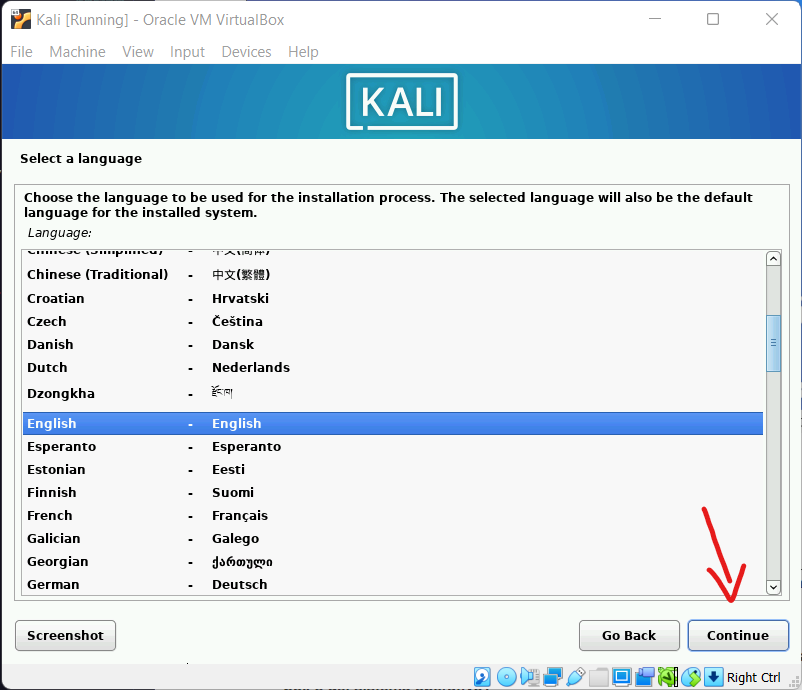
\includegraphics[width = 1\textwidth]{Installation1.png}
        \caption{Siguiendo los pasos (1)}
        \label{fig:Inst1}
    \end{figure}
    \begin{figure} [H]
        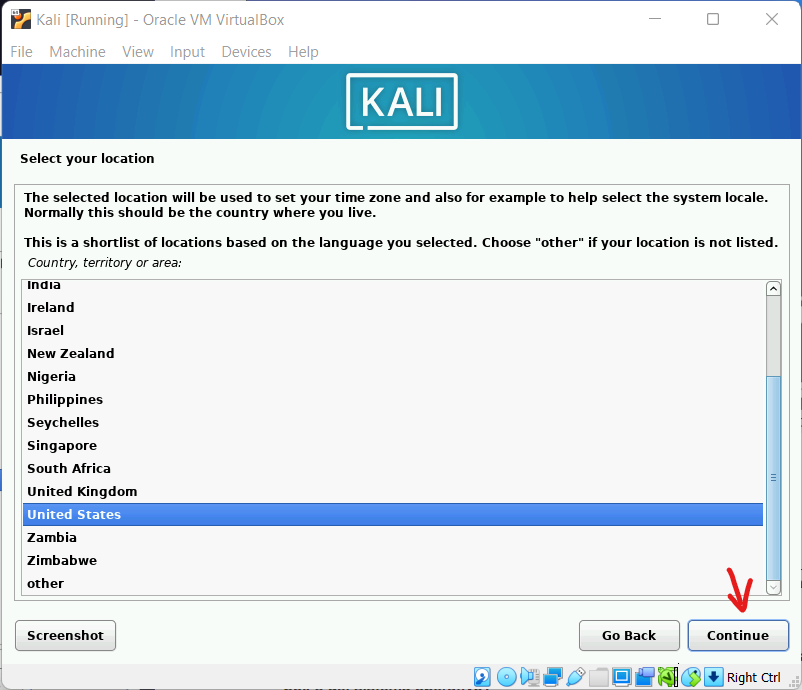
\includegraphics[width = 1\textwidth]{Installation2.png}
        \caption{Siguiendo los pasos (2)}
        \label{fig:Inst2}
    \end{figure}
    \begin{figure} [H]
        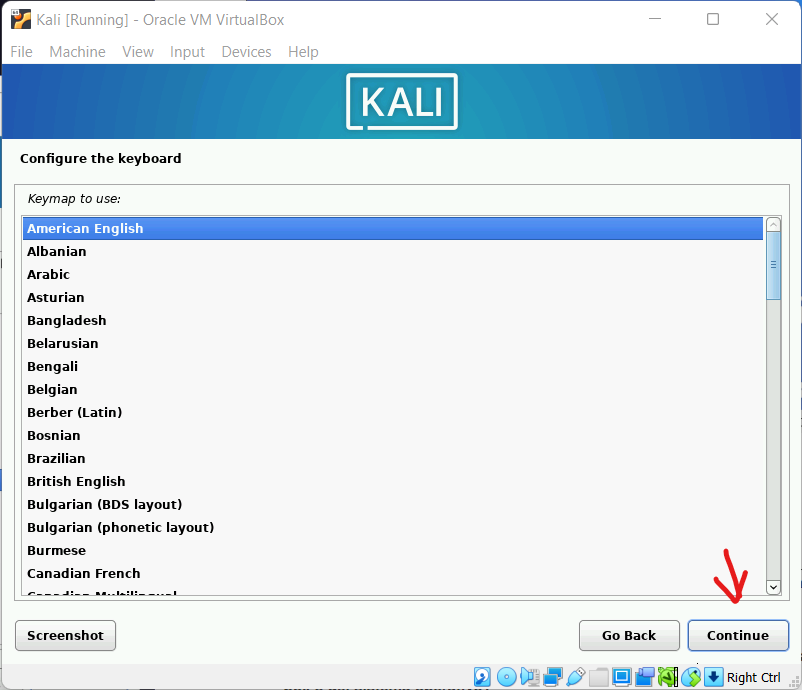
\includegraphics[width = 1\textwidth]{Installation3.png}
        \caption{Siguiendo los pasos (3)}
        \label{fig:Inst3}
    \end{figure}
    \begin{figure} [H]
        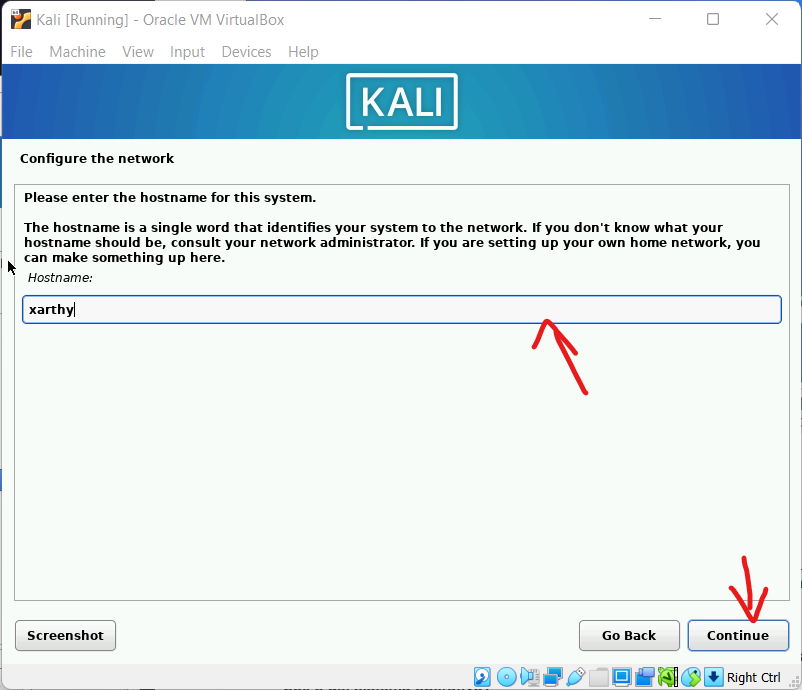
\includegraphics[width = 1\textwidth]{Installation4.png}
        \caption{Siguiendo los pasos (4)}
        \label{fig:Inst4}
    \end{figure}
    \begin{figure} [H]
        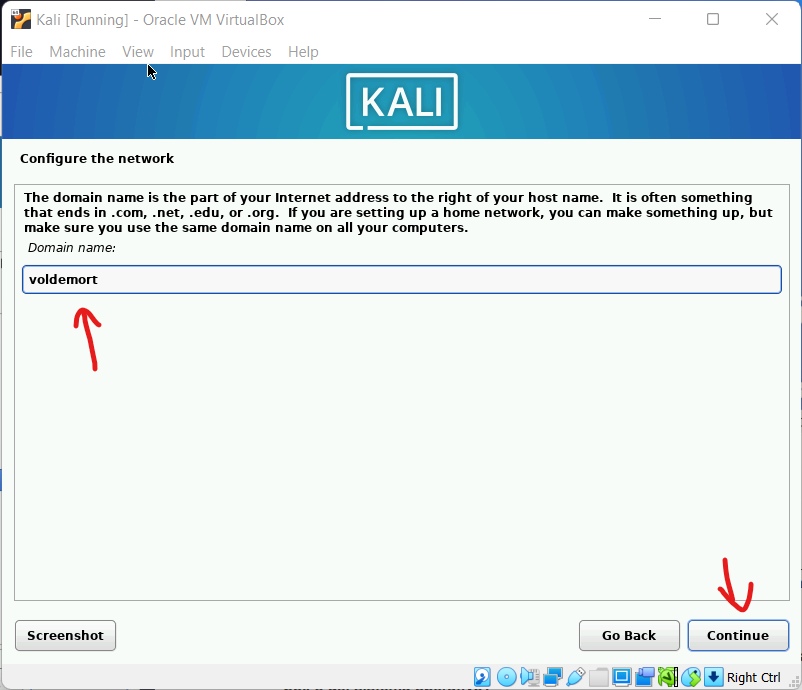
\includegraphics[width = 1\textwidth]{Installation5.png}
        \caption{Siguiendo los pasos (5)}
        \label{fig:Inst5}
    \end{figure}
    \begin{figure} [H]
        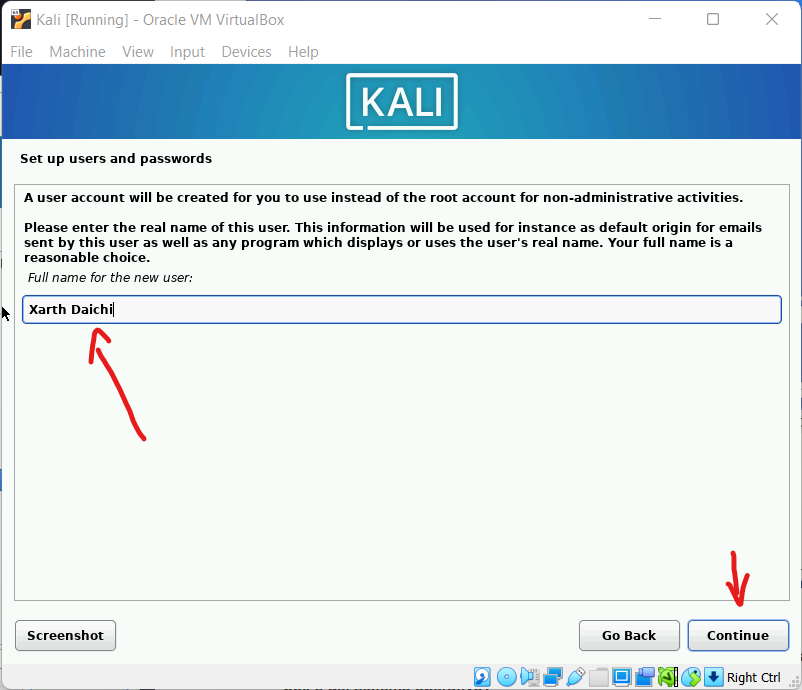
\includegraphics[width = 1\textwidth]{Installation6.png}
        \caption{Siguiendo los pasos (6)}
        \label{fig:Inst6}
    \end{figure}
    \begin{figure} [H]
        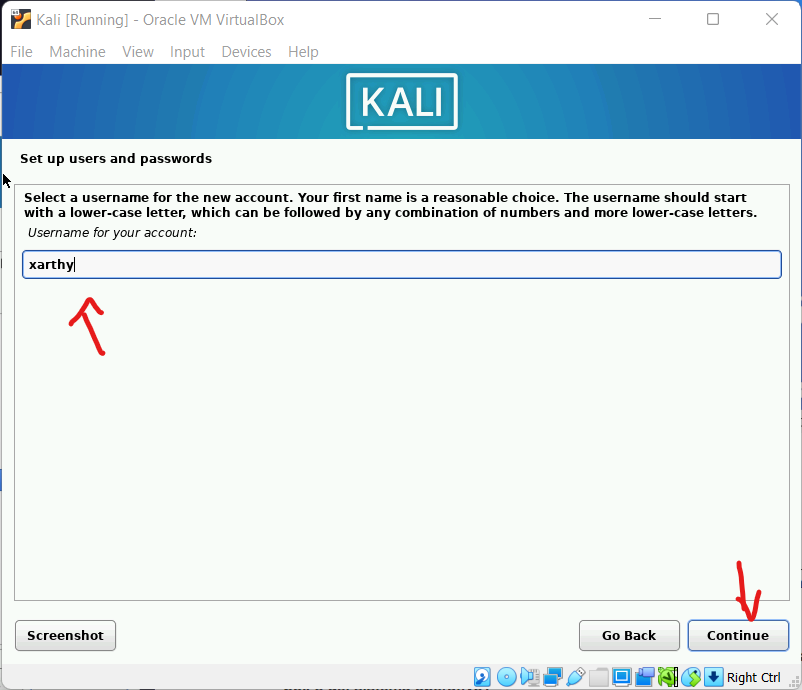
\includegraphics[width = 1\textwidth]{Installation7.png}
        \caption{Siguiendo los pasos (7)}
        \label{fig:Inst7}
    \end{figure}
    \begin{figure} [H]
        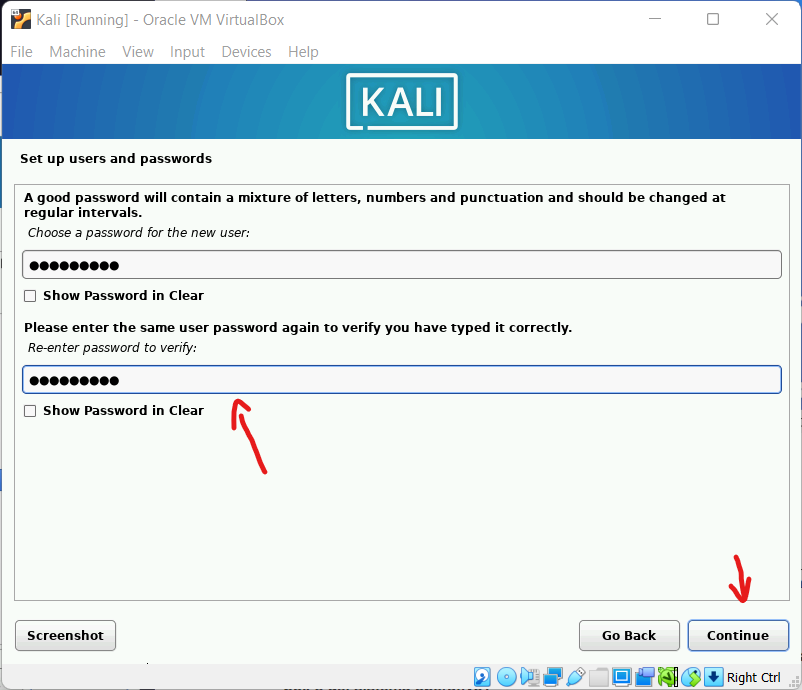
\includegraphics[width = 1\textwidth]{Installation8.png}
        \caption{Siguiendo los pasos (8)}
        \label{fig:Inst8}
    \end{figure}
    \begin{figure} [H]
        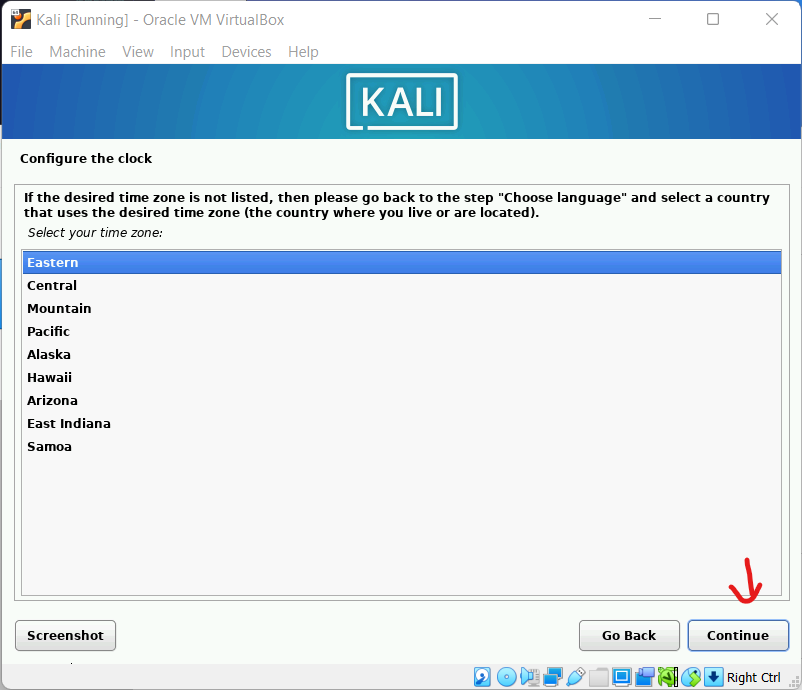
\includegraphics[width = 1\textwidth]{Installation9.png}
        \caption{Siguiendo los pasos (9)}
        \label{fig:Inst9}
    \end{figure}
    \begin{figure} [H]
        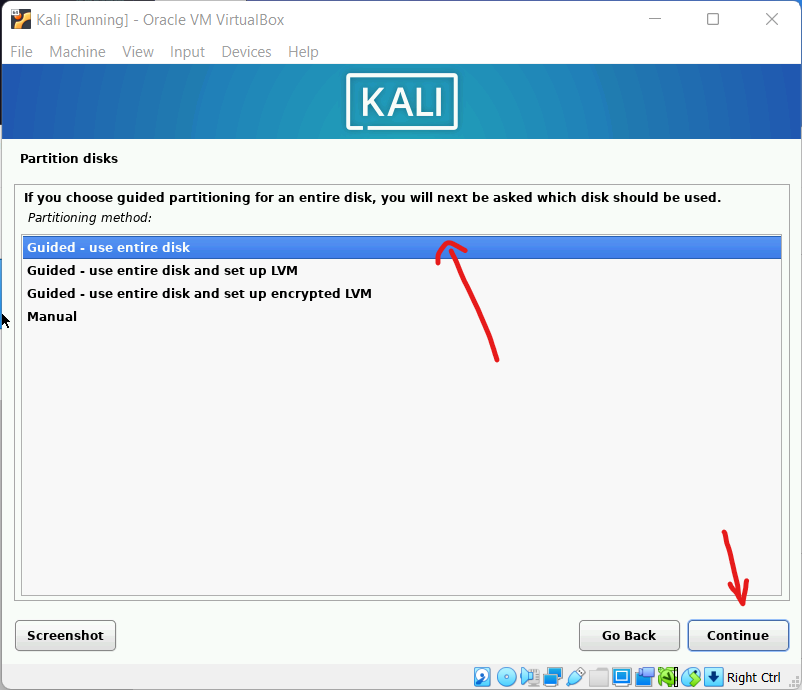
\includegraphics[width = 1\textwidth]{Installation10.png}
        \caption{Siguiendo los pasos (10)}
        \label{fig:Inst10}
    \end{figure}
    \begin{figure} [H]
        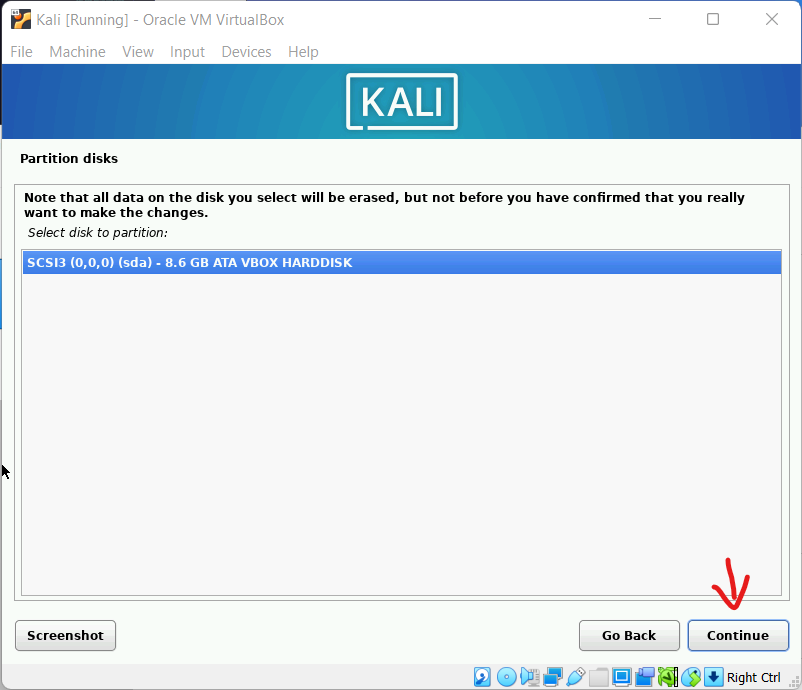
\includegraphics[width = 1\textwidth]{Installation11.png}
        \caption{Siguiendo los pasos (11)}
        \label{fig:Inst11}
    \end{figure}
    \begin{figure} [H]
        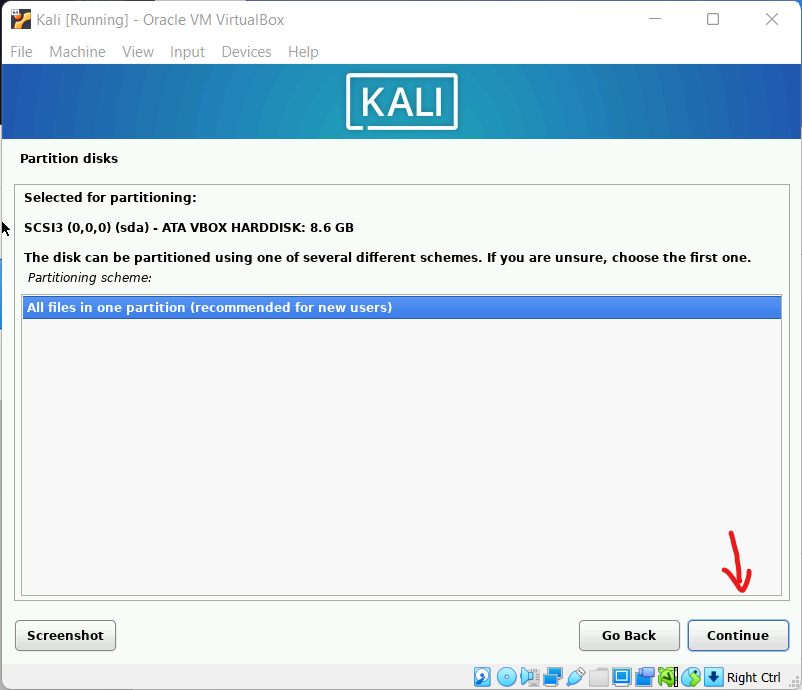
\includegraphics[width = 1\textwidth]{Installation12.png}
        \caption{Siguiendo los pasos (12)}
        \label{fig:Inst12}
    \end{figure}
    \begin{figure} [H]
        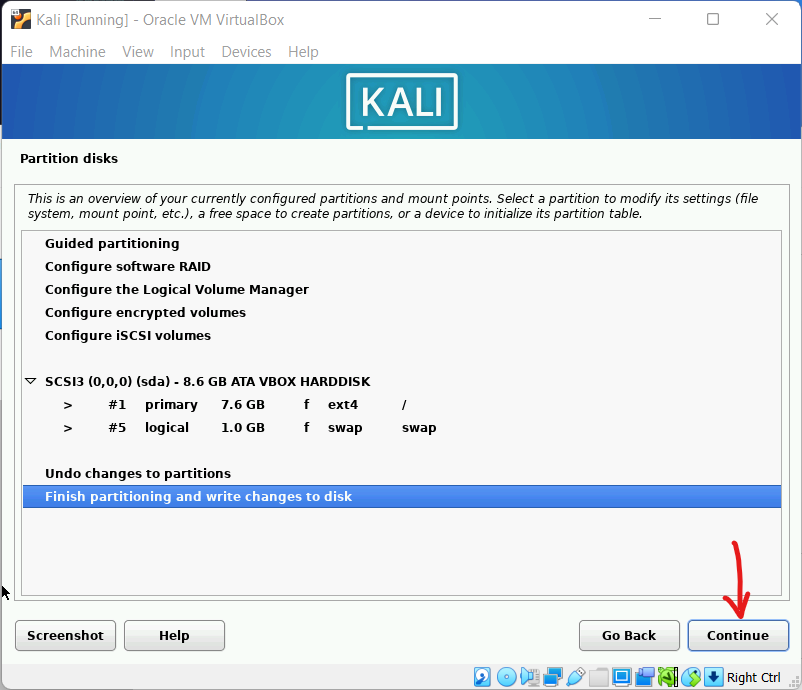
\includegraphics[width = 1\textwidth]{Installation13.png}
        \caption{Siguiendo los pasos (13)}
        \label{fig:Inst13}
    \end{figure}
    \begin{figure} [H]
        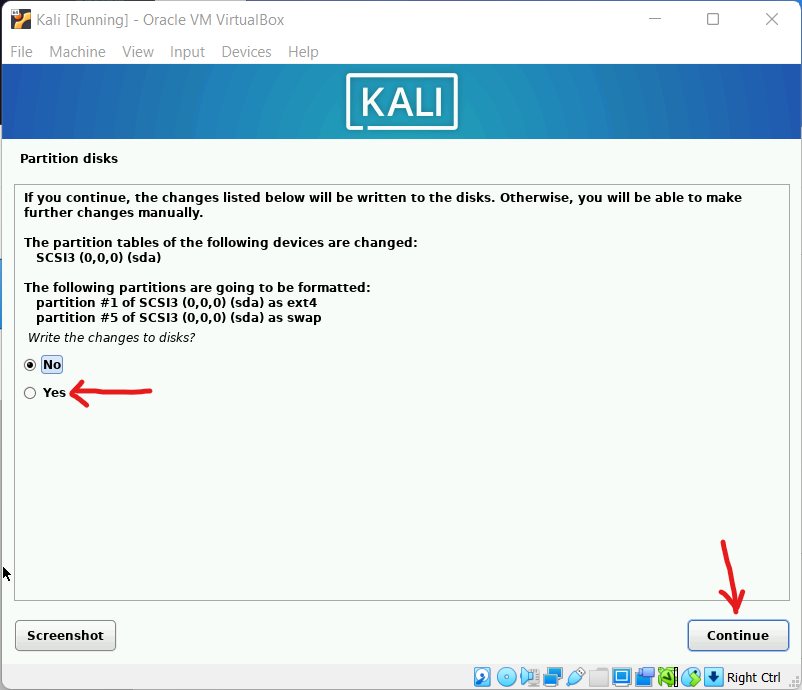
\includegraphics[width = 1\textwidth]{Installation14.png}
        \caption{Siguiendo los pasos (14)}
        \label{fig:Inst14}
    \end{figure}
    \begin{figure} [H]
        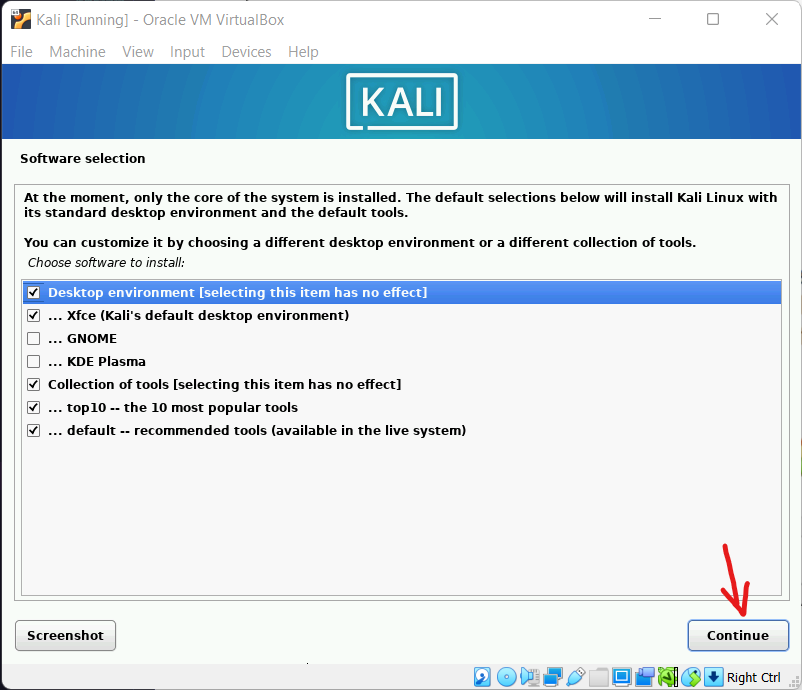
\includegraphics[width = 1\textwidth]{Installation15.png}
        \caption{Siguiendo los pasos (15), para este seleccione el entorno de escritorio favorito}
        \label{fig:Inst15}
    \end{figure}
\end{enumerate}


%------------------------------------------------------------------------------------
\section*{Reporte del laboratorio}
\phantomsection
\addcontentsline{toc}{section}{Reporte del laboratorio}

\begin{itemize}
    \item \textbf{¿Por qué seleccionó la distribución de Linux? Sea específico (a) en esta sección}: Esta fue mi segunda opción personalmente prefiero los sistemas operativos basado en Arch dado a que siento que corren más rápido que los basados en Debian como Ubuntu y PopOs!. Aunque sea basado en Debian Kali es una de las grandes distribuciones para seguridad informática y me gustaría aprender a hacer pentesting (penetration testing) que es ingresar a sistemas, para esto Kali Linux es una buena opción dado a que trae muchas herramientas, en el futuro tal vez experimente con Dark Arch para tener una distribución de seguridad basada en Arch pero de momento estoy usando Kali.
    \item \textbf{¿Tuvo problemas en algún momento del proceso de instalación de virtual box o del sistema operativo?}: Intenté con dos entornos de escritorios de Manjaro, pero por alguna razón me estaba dando un error de Kernel Panic: Terminating idle tasks. Después de buscar la solución cambié la configuración de la máquina virtual para que tuviera dos núcleos y después si me dejó hacer la instalación de Kali.
    \item \textbf{Principales aprendizajes adquiridos}: Ya había experimentado como desde hace aproximadamente 4 años con varias distribuciones de Linux tanto como partición como máquina virtual y hasta WSL. Siempre se aprenden cosas nuevas a la hora de instalar. La primera vez es que tarda un rato y por más que piense que se frenó por lo que más quiera no puedo reiniciar en media instalación. Esta vez aprendí que se requieren varios núcleos para que virtual box funcione correctamente.
    \item \textbf{¿Había instalado una máquina virtual previamente?}: He instalado varias máquinas virtuales tanto con Kali como Pop como Arch solo para ver como se hace y diferentes configuraciones de Arch.
\end{itemize}


%------------------------------------------------------------------------------------
\section*{Conclusión}
\phantomsection
\addcontentsline{toc}{section}{Conclusión}

En conclusión, la máquinas virtuales son programas excelentes que dejan experimentar con varios sistemas operativos y otro tipo de cosas. Entre menos conexiones tiene entre el sistema operativo normal y el de la máquina con mayor seguridad se puede usar, no solo con posibles hackeos (como se encuentra una posibilidad en sitios de pruebas de pentesting), sino que también sirve como una computadora que se puede romper (como Toyota: no lo use maltratelo) y entre menos conexiones menos puede dañar la computadora de verdad. Además se aprendió que a pesar de tener experiencia previa con instalaciones y máquinas siempre se puede encontrar detalles nuevos que aprender.

\newpage
% Referencias
\renewcommand\refname{\large\textbf{Referencias}}
% \bibliography{ref}

\end{document}